% Copyright 2021 Edoardo Riggio

% Licensed under the Apache License, Version 2.0 (the "License");
% you may not use this file except in compliance with the License.
% You may obtain a copy of the License at

% 	http://www.apache.org/licenses/LICENSE-2.0

% Unless required by applicable law or agreed to in writing, software
% distributed under the License is distributed on an "AS IS" BASIS,
% WITHOUT WARRANTIES OR CONDITIONS OF ANY KIND, either express or implied.
% See the License for the specific language governing permissions and
% limitations under the License.

\documentclass{article}

\usepackage{hyperref, amsmath, graphicx, amssymb, csquotes, listings}
\usepackage{fancyvrb,newverbs,xcolor}

\graphicspath{ {./assets/} }

\definecolor{cverbbg}{gray}{0.93}

\newenvironment{cverbatim}
 {\SaveVerbatim{cverb}}
 {\endSaveVerbatim
  \flushleft\fboxrule=0pt\fboxsep=.5em
  \colorbox{cverbbg}{\BUseVerbatim{cverb}}%
  \endflushleft
}

\newenvironment{lcverbatim}
 {\SaveVerbatim{cverb}}
 {\endSaveVerbatim
  \flushleft\fboxrule=0pt\fboxsep=.5em
  \colorbox{cverbbg}{%
    \makebox[\dimexpr\linewidth-2\fboxsep][l]{\BUseVerbatim{cverb}}%
  }
  \endflushleft
}

\newcommand{\ctexttt}[1]{\colorbox{cverbbg}{\texttt{#1}}}
\newverbcommand{\cverb}
  {\setbox\verbbox\hbox\bgroup}
  {\egroup\colorbox{cverbbg}{\box\verbbox}}
  
\lstdefinestyle{c++}{
  frame=single, language={C++}, numbers=left, numberstyle=\tiny, tabsize=4, breaklines=true,
  basicstyle=\ttfamily\scriptsize,
  keywordstyle=\color{blue}\ttfamily,
  otherkeywords={WIDTH},
  keywords=[2]{__shared__},
  keywordstyle=[2]\color{orange}\ttfamily,
  stringstyle=\color{red}\ttfamily,
  commentstyle=\color{green}\ttfamily
}

\begin{document}
\begin{titlepage}
    \begin{center}
        \vspace*{1cm}
        
        \Huge
        \textbf{Artificial Intelligence Cheatsheet}
        
        \vspace{0.5cm}
        \LARGE
        
        \vspace{.5cm}
        
        Edoardo Riggio
   		  \vspace{1.5cm}
       
        \vfill
        
        \today
        
        \vspace{.8cm}
          \Large
          Artificial Intelligence - SA. 2021 \\
        Computer Science\\
        Universit\`{a} della Svizzera Italiana, Lugano\\
        
    \end{center}
\end{titlepage}

\tableofcontents

\newpage

\section{Blind Search Algorithms}
A \textbf{search algorithm} takes as input a problem space and a starting state, and tries to compute a path in the best possible way. \\ \\
The strategy is to search which node to expand among the yet undiscovered nodes. In order to expand a node, we need to consider all of the nodes that are reachable in one step from the selected node.

\subsection{Definitions}
\subsubsection{Search Tree}
A search tree is a tree composed of nodes. Each node in the tree represents a step in the search algorithm. A node is composed of:

\begin{itemize}
	\item State
	\item Node who generated it
	\item Action used to generate it
	\item Depth of the tree
	\item Cost of the path from the root
\end{itemize}

\subsubsection{Travelling Salesman Problem}
The goal of this problem is to visit all the cities of a graph such that the travelling cost is minimum. The travelling cost is measured by summing up all of the travelling costs from the starting city to the destination city.

\subsubsection{Evaluation of Search Strategies}
There are four common criteria for evaluating search strategies:

\begin{itemize}
	\item \textbf{Completeness}
	\vspace{.2cm} \\
	Does the algorithm always find a solution if one exists?
	
	\item \textbf{Optimality}
	\vspace{.2cm} \\
	Does the algorithm guarantee the least-cost solution?
	
	\item \textbf{Time Complexity}
	\vspace{.2cm} \\
	How much time does it take for an algorithm to run?
	
	\item \textbf{Space Complexity}
	\vspace{.2cm} \\
	How much memory does the algorithm require?
\end{itemize}

\subsection{Breath-First Search}
In this algorithm, the shallowest unexpanded node is expanded. In order to do so, this algorithm requires a FIFO queue. This type of queue is able to keep track of which node to expand next. \\

\begin{center}
	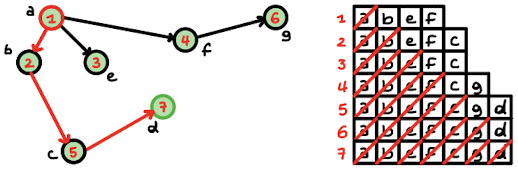
\includegraphics[width=9cm]{bfs.png}
\end{center}
\vspace{.3cm}
This algorithm is \textbf{complete}. It is also \textbf{optimal} in the case that all of the steps have the same cost. Furthermore, the \textbf{space and time complexities} of this algorithm are both $O(b^d)$. Where $b$ is the branching factor, and $d$ is the solution depth.

\subsection{Uniform-Cost Search}
In this algorithm, a cost is assigned to each edge of the graph. Here a node is expanded if $g(n)$ -- i.e. the distance from the root to the node -- is minimal. \\

\begin{center}
	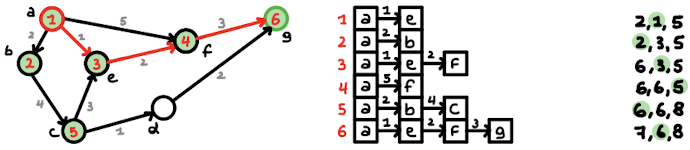
\includegraphics[width=12cm]{ucs.png}
\end{center}
\vspace{.3cm}
In the above image, on the far right we have the values of $g(n)$ at each step, while in the middle, we have the path chosen at each step. \\ \\
This algorithm is \textbf{complete}. It is also \textbf{optimal} in the case that all costs are non-negative. Furthermore, the \textbf{space and time complexities} are both $O(b^d)$, where $b$ is the branching factor, and $d$ is the solution depth.

\subsection{Depth-First Search}
This algorithm expands the deepest unexpanded node. In order to do so, it uses a LIFO queue. \\

\begin{center}
	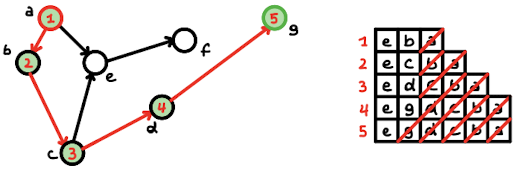
\includegraphics[width=9cm]{dfs.png}
\end{center}
\vspace{.3cm}
This algorithm is \textbf{not complete} in the case of an infinite state space -- since it has no depth limitation. It is also \textbf{not optimal}. Furthermore, the \textbf{time complexity} of the algorithm is $O(b^m)$, while the \textbf{space complexity} is $O(b \cdot m)$. Where $b$ is the branching factor and $m$ is the maximum depth of the search tree.

\subsection{Depth-Limited Search}
In this case we have an algorithm which is identical to the DFS search. The only difference between the two is that depth-limited search is -- as the name suggests -- limited. This means that it will stop when it reaches a certain depth in the solution tree. \\ \\
This algorithm is \textbf{complete} in the case where we know a bound to the solution depth. It is \textbf{not optimal}. Furthermore, the \textbf{time complexity} is $O(b^d)$, and the \textbf{space complexity} is $O(b \cdot d)$. Where $b$ is the branching factor and $d$ is the maximum depth.

\subsection{Iterative Deepening Search}
This is a depth-limited search algorithm, where at each step, a counter representing the tree's depth is incremented. DFS is performed at every repetition of the algorithm -- when the algorithm goes back to the starting node, and it stops at the depth indicated by the counter. \\ \\
This algorithm is \textbf{complete}. It is also \textbf{optimal} in the case that there are non-negative costs. Furthermore, the \textbf{time complexity} is $O(b^d)$, and the \textbf{space complexity} is $O(b \cdot d)$. Where $b$ is the branching factor and $d$ is the depth at which the goal is found.

\subsection{Bi-Directional Search}
This algorithm considers two queues, one only containing the root, and one only containing the goal. The nodes of each queue are expanded until both queues contain a common node. \\ \\
This algorithm is both \textbf{complete} and \textbf{optimal}. Furthermore, the \textbf{time and space complexities} are $O(b ^{\frac{d}{2}})$, where $b$ is the branching factor, and $d$ is the depth at which the goal is located.

\end{document}






























 
